\documentclass{article}
\usepackage{amsmath}
\usepackage{amssymb}
\usepackage{tikz}

\begin{document}

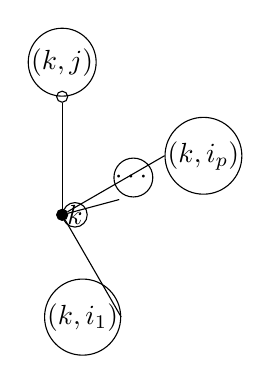
\begin{tikzpicture}[scale=1.5, every node/.style={circle, draw, inner sep=0pt, minimum size=4pt}]
    % Define the coordinates for the nodes
    \node (k) at (0,0) [fill=black] {};
    \node (p) at (0,1) {};
    
    % Draw the edges
    \draw (k) edge (p);
    \draw (k) -- ++(-60:1) node[left] {$(k,i_1)$};
    \draw (k) -- ++( 30:1) node[right] {$(k,i_p)$};
    \draw (k) -- ++( 15:0.5) node[above right, yshift=0.1cm] {$\cdots$};
    
    % Draw the labels for the nodes
    \node at (k) [right] {$k$};
    \node at (p) [above] {$(k,j)$};
\end{tikzpicture}

\end{document}